\chapter{基展开与正则化}

% ============ §5.1 引言 ============
\section{引言}

到目前为止，我们使用的模型——线性回归、LDA、Logistic 回归、分离超平面——全部依赖\textbf{线性模型}。但真实的 $f(X)=\E[Y\mid X]$ 几乎不可能恰好是 $X$ 的线性函数。线性模型只是一种便利的、有时是必须的近似：便利是因为易于解释且是 $f(X)$ 的一阶 Taylor 近似；必须是因为当 $N$ 小或 $p$ 大时，线性模型可能是我们唯一能拟合而不至于过拟合的模型。

本章讨论突破线性局限的核心方法。

\subsection{核心思想：变换输入空间}

用 $X$ 的变换 $h_m(X) : \R^p \to \R$（$m = 1,\ldots,M$）替代或增广原始输入，然后在这些\textbf{派生特征}的新空间中继续使用线性模型：
\begin{equation}\label{eq:basis_expansion}
    f(X) = \sum_{m=1}^{M} \beta_m h_m(X).
\end{equation}

关键在于：一旦基函数 $h_m$ 确定，模型对新变量仍是线性的，所有之前的拟合方法（最小二乘、MLE 等）照常使用。

\subsection{常见基函数示例}

\begin{itemize}
    \item \textbf{恒等变换}：$h_m(X) = X_m$（$m=1,\ldots,p$），还原为原始线性模型。
    \item \textbf{多项式}：$h_m(X) = X_j^2$ 或 $X_j X_k$，实现高阶 Taylor 展开。注意：变量数随阶数指数增长——$p$ 个变量的 $d$ 次多项式需要 $O(p^d)$ 个项。
    \item \textbf{非线性变换}：$h_m(X) = \log(X_j), \sqrt{X_j}, \ldots$，也可使用涉及多个输入的变换如 $\|X\|$。
    \item \textbf{指示函数（分箱）}：$h_m(X) = I(L_m \le X_k < U_m)$，将 $X_k$ 划分为区间，得到分段常数模型。
\end{itemize}

\subsection{复杂度的控制}

基展开产生一个\textbf{字典} $\mathcal{D}$，通常包含大量基函数——远超我们负担得起的数量。控制模型复杂度的方法分为三类：
\begin{itemize}
    \item \textbf{限制法}：限定每个分量函数使用的基函数数量 $M_j$；
    \item \textbf{选择法}：自适应扫描字典，仅包含对拟合有显著贡献的基函数（CART、MARS、boosting 走这条路）；
    \item \textbf{正则化法}：使用整个字典但限制系数（Ridge、Lasso 属于此类）。
\end{itemize}


% ============ §5.2 分段多项式与样条 ============
\section{分段多项式与样条}

本节假设 $X$ 为一维（至 §5.7 放宽）。分段多项式通过将 $X$ 的定义域划分为连续区间、在每个区间内用单独的多项式表示 $f$ 来构造。

\subsection{分段常数与分段线性}

\textbf{分段常数}：三个基函数
\[
h_1(X) = I(X < \xi_1), \quad h_2(X) = I(\xi_1 \le X < \xi_2), \quad h_3(X) = I(\xi_2 \le X),
\]
最小二乘估计 $\hat{\beta}_m = \bar{Y}_m$（第 $m$ 区间的 $Y$ 均值）。

\textbf{分段线性}：需要额外三个基函数 $h_{m+3} = h_m(X)X$（$m=1,2,3$），共 6 个参数。但通常我们希望函数在节点 $\xi_1, \xi_2$ 处\textbf{连续}——连续性约束 $f(\xi_1^-) = f(\xi_1^+)$ 和 $f(\xi_2^-) = f(\xi_2^+)$ 各消耗一个自由度，剩下 4 个自由参数。

\begin{figure}[htbp]
\centering
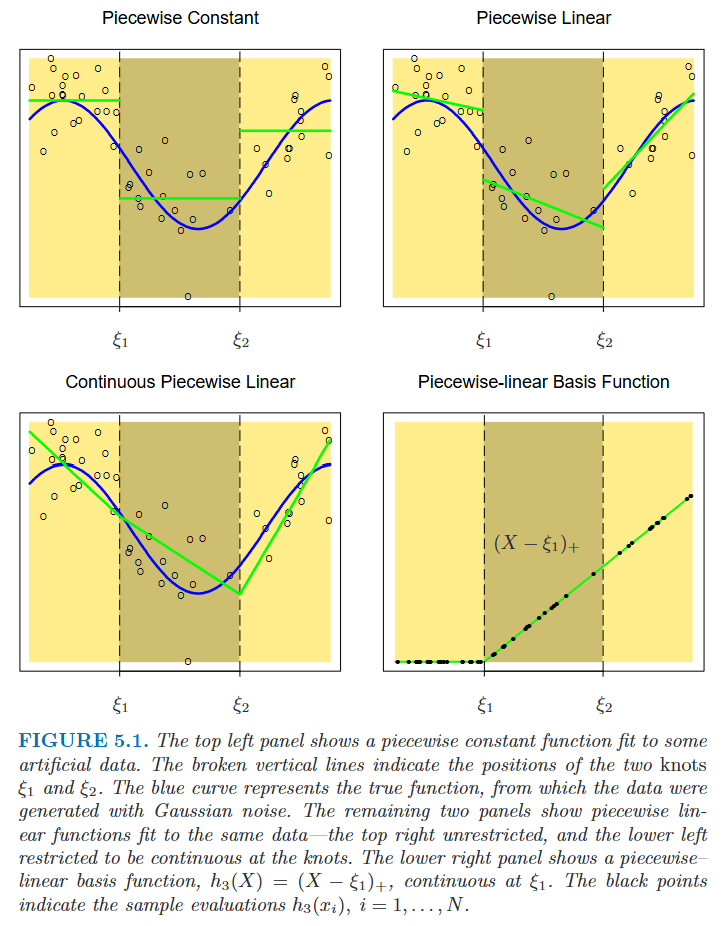
\includegraphics[width=0.9\textwidth]{Chapters/pic/ch_基展开和正则化/figure_5_1.png}
\caption{分段多项式拟合人造数据。左上：分段常数（三个区间各自的均值）；右上：无约束分段线性；左下：节点处连续的分段线性；右下：截断幂基函数 $h_3(X)=(X-\xi_1)_+$（在 $\xi_1$ 之前为 0，之后线性增长）。来源：ESL Figure 5.1。}
\label{fig:piecewise}
\end{figure}

\subsection{截断幂基}

更直接的方式是使用内建了连续性约束的基函数：
\[
h_1(X)=1,\; h_2(X)=X,\; h_3(X)=(X-\xi_1)_+,\; h_4(X)=(X-\xi_2)_+,
\]
其中 $(X-\xi)_+ = \max(0, X-\xi)$ 为\textbf{截断幂函数}。

\textbf{截断幂函数的直观}：$(X-\xi)_+$ 在 $\xi$ 之前恒为 0（「关着」），在 $\xi$ 之后是一条斜率为 1 的直线（「打开」）。在 $\xi$ 处值为 0，故连续但导数不连续（有个「折角」）。用截断幂函数构造分段线性模型的逻辑为：
\[
f(X) = \beta_0 + \beta_1 X + \beta_2 (X-\xi_1)_+ + \beta_3 (X-\xi_2)_+.
\]
\begin{itemize}
    \item $X < \xi_1$：只有 $\beta_0 + \beta_1 X$（一条直线）；
    \item $\xi_1 \le X < \xi_2$：$(X-\xi_1)_+$ 打开 → 斜率从 $\beta_1$ 变为 $\beta_1+\beta_2$（拐弯了）；
    \item $X \ge \xi_2$：$(X-\xi_2)_+$ 也打开 → 斜率再变一次。
\end{itemize}
每个截断幂函数在对应节点处添加一个「拐弯」，不影响节点左侧，只改变右侧行为。这比显式施加连续性约束更加自然。

更高次幂的推广：$(X-\xi)_+^2$ 在节点处有一阶连续导数（光滑拐弯），$(X-\xi)_+^3$ 在节点处有二阶连续导数（人眼无法察觉拐弯）。

\begin{remark}
有人可能会问：为什么 $(X-\xi_1)_+$ 在第二、第三区间都开着，而不设计成只在 $[\xi_1,\xi_2)$ 上非零？答案是为了\textbf{保证连续性}——如果在 $\xi_2$ 处强行把它关掉（变为 0），函数值会突然跳变，破坏连续性。截断幂基的「全局影响」是换取系数可解释性的代价（$\beta_j$ 直接对应「第 $j$ 个节点处的斜率变化量」）。若需要只在局部非零的基函数，可用\textbf{B-样条 (B-splines)}——每个 B-样条基函数只在有限几个区间上非零（局部支撑），数值更稳定，但系数不再有截断幂基那样的直观解释。
\end{remark}

\subsection{三次样条 (Cubic Spline)}

分段三次多项式，在节点处具有连续的一阶和二阶导数（$M=4$ 阶样条）。可视作：
\begin{center}
\begin{tabular}{c|c|c}
\hline
阶数 & 连续性 & 名称 \\
\hline
$M=1$ & 无连续要求 & 分段常数 \\
$M=2$ & 连续，导数不连续 & 线性样条（连续分段线性） \\
$M=4$ & 二阶导数连续 & 三次样条 \\
\hline
\end{tabular}
\end{center}

\begin{figure}[htbp]
\centering
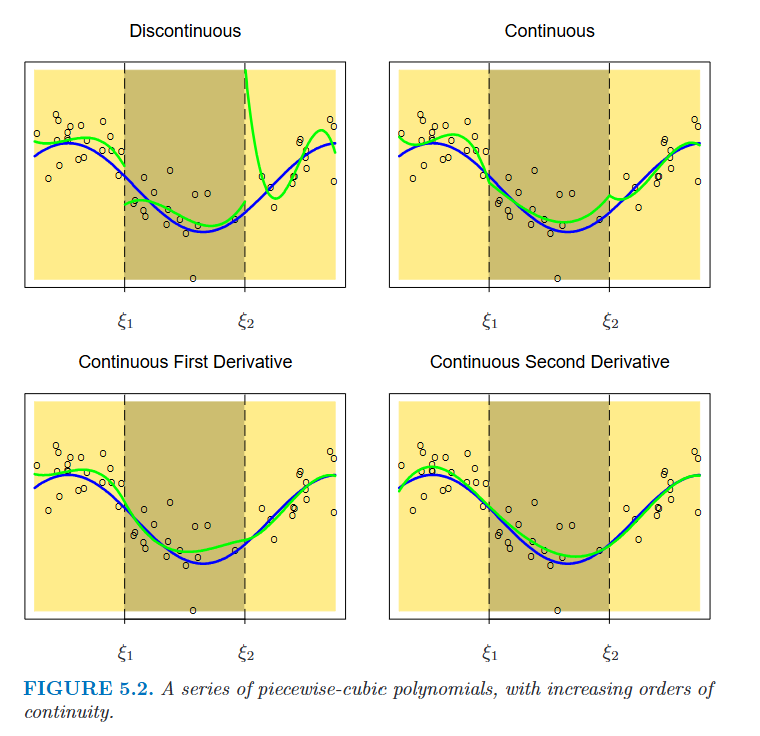
\includegraphics[width=0.9\textwidth]{Chapters/pic/ch_基展开和正则化/figure_5_2.png}
\caption{分段三次多项式，节点处连续性递增。左上：不连续；右上：连续但导数不连续；左下：一阶导数连续；右下：一阶和二阶导数均连续（三次样条）。再额外施加一阶连续性将退化为全局三次多项式。来源：ESL Figure 5.2。}
\label{fig:cubic_splines}
\end{figure}

对于节点 $\xi_1, \xi_2$，三次样条的一个基础表示（截断幂基）：
\begin{equation}\label{eq:cubic_spline_basis}
    \begin{aligned}
    h_1(X) &= 1, \quad h_2(X) = X, \quad h_3(X) = X^2, \\
    h_4(X) &= X^3, \quad h_5(X) = (X-\xi_1)_+^3, \quad h_6(X) = (X-\xi_2)_+^3.
    \end{aligned}
\end{equation}
共 6 个基函数对应 6 维线性函数空间。参数计数验证：3 个区域 $\times$ 每区域 4 参数 $-$ 2 个节点 $\times$ 每节点 3 个约束 $= 6$。

\subsection{一般阶样条}

\textbf{$M$（阶数）的含义}：$M = \text{次数} + 1$，即每个区间内多项式的参数个数。

\begin{center}
\begin{tabular}{c|c|c|c}
\toprule
$M$ & 次数 & 名称 & 连续性 \\
\midrule
1 & 0 次（常数） & 分段常数 & 无 \\
2 & 1 次（线性） & 线性样条 & $f$ 连续 \\
3 & 2 次（二次） & 二次样条 & $f, f'$ 连续 \\
4 & 3 次（三次） & 三次样条 & $f, f', f''$ 连续 \\
\bottomrule
\end{tabular}
\end{center}

$M$ 阶样条是 $M$ 阶分段多项式，且在节点处有直到 $M-2$ 阶的连续导数。带 $K$ 个节点 $\xi_j$ 的截断幂基一般形式为：
\begin{equation}\label{eq:truncated_power}
    \begin{aligned}
    h_j(X) &= X^{j-1}, \quad j = 1,\ldots,M, \\
    h_{M+\ell}(X) &= (X - \xi_\ell)_+^{M-1}, \quad \ell = 1,\ldots,K.
    \end{aligned}
\end{equation}
即 $M$ 个全局多项式基函数 + $K$ 个节点处的截断幂基函数，共 $M+K$ 个。

\textbf{自由度的计算}：
\[
\boxed{\mathrm{df} = M + K.}
\]
推导：$(K+1)$ 个区间 $\times$ 每区间 $M$ 个系数 $-$ $K$ 个节点 $\times$ 每节点 $M-1$ 个连续性约束 $= M(K+1) - K(M-1) = M+K$。

具体示例：
\begin{center}
\begin{tabular}{c|c|c|c}
\toprule
样条类型 & $M$ & 节点数 $K$ & df \\
\midrule
分段常数 & 1 & 2 & 3 \\
线性样条 & 2 & 2 & 4 \\
三次样条 & 4 & 2 & 6 \\
自然三次样条 & 4 & $K$ & $K$（$4+K$ 减去边界 4 个约束） \\
\bottomrule
\end{tabular}
\end{center}

在 R 中，\texttt{bs(x, df=7)} 的内部逻辑：三次样条 $M=4$，故内节点数 $= 7-4 = 3$（加 3 个边界节点共 6 个节点），放于适当的分位数处。

\textbf{实践中最常用的阶数}：$M=1,2,4$。三次样条是最低阶的「人眼看不见节点处不连续」的样条——极少有理由使用更高阶。

\begin{remark}
截断幂基在概念上简单，但数值上不稳健——大数的幂会导致严重舍入误差。实际计算中普遍使用\textbf{B-样条基}（见本章附录），它具有更好的数值稳定性且计算高效。
\end{remark}

\subsection{节点选择}

\subsubsection{R 中的实现}

ESL 全书使用统计编程语言 R 做代码示例。\texttt{bs(x, df=7)} 是 R 的 \texttt{splines} 包中的函数：输入向量 $x$，输出 $N \times 7$ 的 B-样条基矩阵。Python 中类似功能由 \texttt{scipy.interpolate.BSpline} 或 \texttt{patsy.dmatrix} 提供。

内部逻辑：三次样条 $M=4$，故 \texttt{df=7} → 内节点数 $= 7-4 = 3$，自动放置在 $x$ 的 25\%, 50\%, 75\% 分位数处（加上边界节点构成完整节点集）。

\subsubsection{实践中节点位置怎么选？}

\textbf{标准做法——不看节点位置，只选 df}。实践中几乎不手动指定节点位置，而是通过交叉验证选择 df（自由度 ≈ 复杂度），让函数自动放置节点：

\begin{center}
\begin{tabular}{c|c}
\toprule
df & 模型含义 \\
\midrule
1 & 常数（仅截距） \\
2 & 直线（截距 + 斜率） \\
4 & 很光滑的非线性 \\
7 & 中等弯曲 \\
12 & 相当灵活 \\
\bottomrule
\end{tabular}
\end{center}

df 越大 → 节点越多 → 模型越灵活 → 偏差↓、方差↑。通过 $K$ 折交叉验证选择使测试误差最小的 df。

\textbf{默认分位数放置的启发式原理}：R 将节点放在 $x$ 的均匀分位数处（而不是等间距）。直觉是——数据密集的地方需要更多灵活性来捕捉信号，数据稀疏的地方不宜浪费自由度拟合噪声。这并非数学最优（本节末尾讨论），但在绝大多数实际问题中足够好用。

\textbf{特定场景的调整}：
\begin{itemize}
    \item 有领域知识时：在已知的物理拐点（如材料相变温度、药物半衰期）处手动放置节点；
    \item 自然样条：边界外线性约束 → 边界节点靠近数据极值，内部节点均匀分位数；
    \item 周期性数据：改用周期样条基（Fourier 基或周期 B-样条）。
\end{itemize}

\subsubsection{分位数放置是最优的吗？}

不是。最优节点选择是组合优化问题——从 $N$ 个数据点中选 $K$ 个节点有 $\binom{N}{K}$ 种可能，NP-hard。

分位数放置只是一个统计上稳健的启发式，原理是「在数据多的地方多放节点」。真正试图优化节点位置的方法：
\begin{itemize}
    \item \textbf{MARS（§9.4）}：贪心添加 + 剪枝，自适应搜索节点位置；
    \item \textbf{穷举/贪心搜索}：计算量过大，$K>3$ 时不可行。
\end{itemize}

实践结论：\textbf{没人手动调节点位置。}标准做法是用 \texttt{bs(x, df=k)}，$k$ 由 CV 决定，分位数自动放置节点。这套组合虽非数学最优，但在偏差-方差权衡下统计上稳健。真正花精力搜索最优节点的方法反而不如大量节点 + 惩罚（光滑样条，§5.4）实用。

标准三次样条在边界区域方差爆增（图 5.3）。\textbf{自然三次样条}添加额外约束：函数在边界节点之外是\textbf{线性的}。这释放了 4 个自由度（两个边界区域各两个约束），可重新分配到内部区域增加节点。

带 $K$ 个节点的自然三次样条由 $K$ 个基函数表示。从截断幂基出发施加边界约束，可得基函数（习题 5.4）：
\begin{equation}\label{eq:natural_spline_basis}
    N_1(X) = 1,\quad N_2(X) = X,\quad N_{k+2}(X) = d_k(X) - d_{K-1}(X),
\end{equation}
其中
\[
d_k(X) = \frac{(X - \xi_k)_+^3 - (X - \xi_K)_+^3}{\xi_K - \xi_k}.
\]
每个基函数在 $X \ge \xi_K$ 处二阶和三阶导数均为零。

\textbf{权衡}：边界附近偏差略有增加（假设函数在边界处近似线性通常是合理的），但方差大幅降低。

\subsection{样条方法概览}

在进入具体实例之前，对目前以及后续出现的样条方法做一个系统总结：

\begin{center}
\small
\begin{tabular}{llll}
\toprule
类型 & 节点 & 复杂度控制 & 特点 \\
\midrule
回归样条（§5.2） & 手动选 $K$ 个内节点 & $\mathrm{df}=M+K$ & 最基础 \\
自然样条（§5.2.1） & 同上 + 边界线性约束 & $\mathrm{df}=K$ & 降边界方差，最常用 \\
B-样条（附录） & 同回归样条 & 同回归样条 & 局部支撑，数值稳定 \\
周期样条 & 同上 + 循环边界 & 同上 & 周期性数据 \\
光滑样条（§5.4） & 每个 $x_i$ 都是节点 & $\lambda$ 惩罚 $\int(f'')^2$ & 免选节点，$\lambda$ 由 CV 定 \\
惩罚样条 (P-splines) & 均匀密节点 + 差分惩罚 & $\lambda$ 惩罚系数差 & 更高效，现代 GAM 主流 \\
薄板样条（§5.7） & 多维推广 & $\lambda$ 惩罚曲率 & 多维光滑样条 \\
张量积样条 & 多维交互 & 基数 $=$ 各维基数的乘积 & 建模联合非线性 \\
MARS（§9.4） & 自适应选择 & 贪心 + 剪枝 & 自动找交互和节点 \\
\bottomrule
\end{tabular}
\end{center}

本章重点介绍回归样条（§5.2）、自然样条（§5.2.1）和光滑样条（§5.4），后续各章将逐步展开其余方法。读者可随时回查此表以保持方向感。

\subsection{示例：南非心脏病数据（续）}

\subsubsection{问题设定}

将 §4.4.2 的南非心脏病回顾性调查重新考察。数据概要：
\begin{itemize}
    \item \textbf{响应 $Y$}：二分类——是否患有心肌梗死 (MI/chd)，$Y=1$（患病/病例），$Y=0$（未患病/对照）；
    \item \textbf{特征 $X$}：7 个风险因子——\texttt{sbp}（收缩压）、\texttt{tobacco}（累计烟龄，kg）、\texttt{ldl}（坏胆固醇）、\texttt{famhist}（家族史：有/无）、\texttt{obesity}（肥胖指数）、\texttt{alcohol}（饮酒量）、\texttt{age}（年龄）；
    \item \textbf{样本量}：$N=462$（160 病例 + 302 对照）。
\end{itemize}

\subsubsection{第一步：线性 Logistic 回归 → 确定谁不显著}

先用线性 Logistic 回归（§4.4.2，表 4.2）拟合并做 Wald 检验。Z 得分 $= \hat{\beta}_j / \text{SE}(\hat{\beta}_j)$（系数除以其标准误），$\vert Z\vert > 2 \approx p<0.05$ 表示显著。结果：
\[
\begin{array}{c|c|c|c}
\text{变量} & \hat{\beta} & \text{SE} & Z \\ \hline
\text{sbp} & 0.006 & 0.006 & 1.02\;\text{不显著} \\
\text{tobacco} & 0.080 & 0.026 & 3.03\;\text{显著} \\
\text{ldl} & 0.185 & 0.057 & 3.22\;\text{显著} \\
\text{famhist} & 0.939 & 0.225 & 4.18\;\text{显著} \\
\text{obesity} & -0.035 & 0.029 & -1.19\;\text{不显著} \\
\text{age} & 0.043 & 0.010 & 4.18\;\text{显著}
\end{array}
\]

在线性模型中，\textbf{sbp 和 obesity 被判为「没有用」——会被剔除}。但直觉上血压和肥胖应该与心脏病相关——可能线性假设太强了。

\subsubsection{第二步：改用自然样条 → 允许非线性效应}

对每个连续变量 $X_j$，用 4 个自然样条基函数（对应 3 个内节点放在 $X_j$ 的均匀分位数处）替代原始 $X_j$：
\begin{equation}\label{eq:spline_logistic}
    \operatorname{logit}[\Pr(\text{chd}\mid X)] = \theta_0 + h_1(X_1)^\top\theta_1 + \cdots + h_p(X_p)^\top\theta_p,
\end{equation}
其中每个 $h_j(X_j)$ 是 $X_j$ 处 4 个自然样条基函数的取值向量，$\theta_j$ 是 4 维系数向量。二值因子 \texttt{famhist} 仍用哑变量编码（1 个参数）。

\textbf{关键区别}：线性模型中 sbp 的效应是 $\beta_{\text{sbp}} \times \text{sbp}$（一条直线，一个系数）；样条模型中 sbp 的效应是 $f_{\text{sbp}}(\text{sbp}) = h(\text{sbp})^\top\theta_{\text{sbp}}$（一条曲线，4 个系数共同决定形状）。图 5.4 中每个面板画的正是 $\hat{f}_j(X_j)$——第 $j$ 个变量对 log-odds 的（非线性的）估计贡献函数。

$f_j(X_j)$ 的计算方式：将所有 $p$ 组基函数（加常数项）合并为大向量 $h(X)$，总参数 $\mathrm{df}=1+\sum_j\mathrm{df}_j$。评在 $N$ 个样本上得 $N\times\mathrm{df}$ 基矩阵 $\mathbf{H}$，用 §4.4.1 的 IRLS 算法拟合 Logistic 回归得 $\hat{\theta}$，然后 $f_j$ 在任意 $X_j$ 处的值由 $h_j(X_j)^\top\hat{\theta}_j$ 计算。

\subsubsection{第三步：模型选择与最终结果}

执行向后逐步删除，保留项的组结构（一次删除整组基函数而非单个系数），用 AIC 统计量（§7.5）决定。最终模型见 Figure 5.4 和 Table 5.1。

\begin{figure}[htbp]
\centering
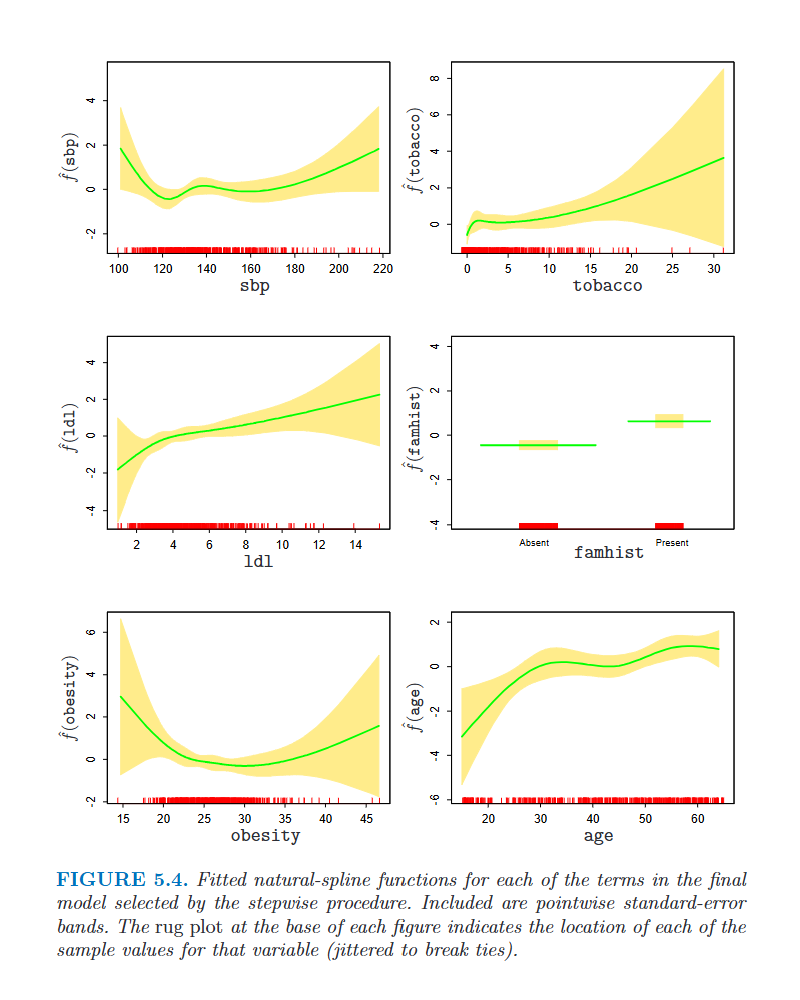
\includegraphics[width=0.95\textwidth]{Chapters/pic/ch_基展开和正则化/figure_5_4.png}
\caption{最终模型中各变量的拟合自然样条函数。实线：$\hat{f}_j(X_j)$；虚线带：$\pm 2$ 标准误的逐点置信带；底部 rug plot：每个刻度对应一个样本在该变量上的取值（抖动防重叠）。famhist 为二值变量，显示为两个点 + 误差棒。来源：ESL Figure 5.4。}
\label{fig:heart_splines}
\end{figure}

\textbf{Figure 5.4 读法}：六个面板，每个对应一个变量。
\begin{itemize}
    \item \textbf{实线} = $\hat{f}_j(X_j)$——该变量对 log-odds 的非线性估计效应。弯曲 = 非线性，平直 = 线性够用；
    \item \textbf{虚线带} = $\pm 2$ 标准误的逐点置信带——带越宽，估计越不确定（数据稀疏处自然宽）；
    \item \textbf{底部 rug plot} = 每个刻度是一个样本在该变量上的取值——刻度密 → 数据多 → 曲线可信；
    \item \textbf{famhist 面板}：二值变量，显示为两个点 + 误差棒（有/无家族史 ⇒ 增加约 0.5 个 log-odds 单位的风险）。
\end{itemize}

\begin{figure}[htbp]
\centering
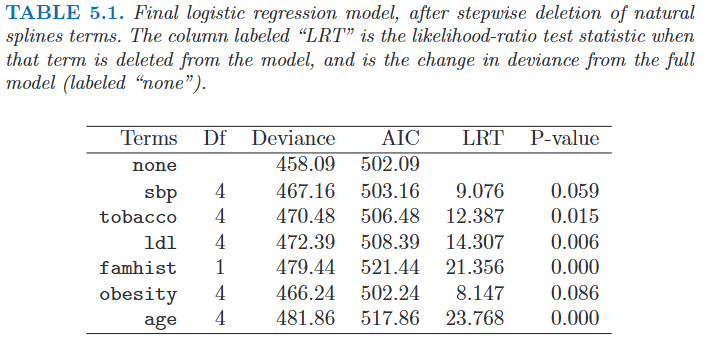
\includegraphics[width=0.85\textwidth]{Chapters/pic/ch_基展开和正则化/table_5_1.png}
\caption{逐步删除自然样条项后的最终 Logistic 回归模型。Terms：变量名（none=全模型）；Df：该变量占用自由度；Deviance：离差；AIC：赤池信息准则；LRT：似然比检验统计量（该变量删除后 deviance 的增加量）；P-value：LRT 的 p 值。来源：ESL Table 5.1。}
\label{tab:heart_final}
\end{figure}

\textbf{Table 5.1 读法（以 sbp 行为例）}：
\begin{center}
\begin{tabular}{cccccc}
\toprule
Terms & Df & Deviance & AIC & LRT & P-value \\
\midrule
none（全模型） & — & 458.09 & 502.09 & — & — \\
sbp（删除后） & 4 & 467.16 & 503.16 & 9.076 & 0.059 \\
\bottomrule
\end{tabular}
\end{center}
\begin{itemize}
    \item \textbf{Df}：该变量占用的自由度（连续变量 = 4 个样条基函数；famhist = 1 个哑变量）；
    \item \textbf{Deviance}：删除该变量后模型的离差（$=-2\times$ 对数似然，类比 RSS）；
    \item \textbf{AIC}：Deviance + 2×df 的惩罚（越小越好）；
    \item \textbf{LRT（似然比检验）} = $\text{Deviance}_{\text{删除后}} - \text{Deviance}_{\text{全模型}}$：衡量删除该变量造成的拟合损失。越大 ⇒ 变量越重要；
    \item \textbf{P-value}：LRT 的 p 值，$<0.05$ ⇒ 显著（不能删）。sbp 的 p=0.059，接近显著但刚好过线——作者选择保留。
\end{itemize}

\textbf{按重要性排名（LRT 从大到小）}：$\text{age}(23.8) > \text{famhist}(21.4) > \text{ldl}(14.3) > \text{tobacco}(12.4) > \text{sbp}(9.1) > \text{obesity}(8.1)$。

\subsubsection{关键发现与解释}

\textbf{sbp}（收缩压）和 \textbf{obesity}（肥胖）在线性模型中不显著（Z 得分 $\approx 1$），但在样条模型中\textbf{被保留下来}——因为它们的贡献本质上是非线性的（图 5.4 显示 U 形效应：低值和高值均增加风险）。这正是基展开超越线性的实际价值：\textbf{「直线工具太钝，切不出曲线」——换样条这把更灵活的工具，真实的非线性效应才得以显现。}

低值区域出现风险上升看似反常（血压低/体重轻反而风险高？），但这是回顾性数据的体现：患者心梗发作后已受益于健康饮食和生活方式改变（血压降低了、体重减轻了），导致低 sbp/obesity 区域的表面风险升高——因果方向被数据收集方式反转。

\subsubsection{数学推导：$\hat{f}_{\mathrm{sbp}}(x)$ 如何计算}

以 sbp 为例，用严格的符号语言揭示图 5.4 的完整计算链。

\textbf{Step 1——构造基函数}：对 sbp 选取 $K=5$ 个节点（2 个边界 = $\min$ 和 $\max$，3 个内节点放在样本分位数处），4 个自然三次样条基函数为（\eqref{eq:natural_spline_basis}）：
\[
h_1(x)=1,\quad h_2(x)=x,\quad h_3(x)=d_1(x)-d_{K-1}(x),\quad h_4(x)=d_2(x)-d_{K-1}(x),
\]
其中 $d_k(x)=\frac{(x-\xi_k)_+^3-(x-\xi_K)_+^3}{\xi_K-\xi_k}$（每 $d_k$ 保证在 $x\ge\xi_K$ 处三阶导数为零）。

\textbf{Step 2——构造 sbp 的设计矩阵}：对 $i=1,\ldots,N$，第 $i$ 个样本的 sbp 值为 $x_{i,\mathrm{sbp}}$，其对应的 $1\times 4$ 基向量为：
\[
h_{\mathrm{sbp}}(x_{i,\mathrm{sbp}}) = [h_1(x_{i,\mathrm{sbp}}),\; h_2(x_{i,\mathrm{sbp}}),\; h_3(x_{i,\mathrm{sbp}}),\; h_4(x_{i,\mathrm{sbp}})].
\]
所有 7 个变量的基函数 + 常数项合并为 $\mathbf{H}_{N\times\mathrm{df}}$，其中 sbp 对应的 4 列为第 $k_{\mathrm{sbp}}+1$ 到 $k_{\mathrm{sbp}}+4$ 列。

\textbf{Step 3——拟合 Logistic 回归}：用 IRLS（§4.4.1）最大化对数似然，得参数估计 $\hat{\theta}\in\R^{\mathrm{df}}$。sbp 对应的 4 个系数为子向量 $\hat{\theta}_{\mathrm{sbp}} = (\hat{\theta}_{\mathrm{sbp},1}, \ldots, \hat{\theta}_{\mathrm{sbp},4})^\top$。

\textbf{Step 4——在任意值 $x$ 处计算 $\hat{f}_{\mathrm{sbp}}(x)$}：
\[
\boxed{\hat{f}_{\mathrm{sbp}}(x) = \sum_{m=1}^{4} \hat{\theta}_{\mathrm{sbp},m}\; h_m(x)
    = h_{\mathrm{sbp}}(x)^\top \hat{\theta}_{\mathrm{sbp}}.}
\]
在 sbp 的值域上取均匀网格 $\{x_1,\ldots,x_{100}\}$，逐点计算即得图 5.4 中的实线。

\textbf{Step 5——置信带的计算}：$\hat{\theta}$ 的渐近协方差矩阵为 $\widehat{\operatorname{Cov}}(\hat{\theta}) = (\mathbf{H}^\top\mathbf{W}\mathbf{H})^{-1}$（从 IRLS 最后一轮获得）。取 sbp 对应的 $4\times 4$ 子块 $\widehat{\operatorname{Cov}}(\hat{\theta}_{\mathrm{sbp}})$，则在 $x$ 处 $\hat{f}_{\mathrm{sbp}}(x)$ 的标准误为：
\[
\operatorname{SE}[\hat{f}_{\mathrm{sbp}}(x)] = \sqrt{h_{\mathrm{sbp}}(x)^\top\; \widehat{\operatorname{Cov}}(\hat{\theta}_{\mathrm{sbp}})\; h_{\mathrm{sbp}}(x)}.
\]
图中虚线带即为 $\hat{f}_{\mathrm{sbp}}(x) \pm 2\cdot\operatorname{SE}[\hat{f}_{\mathrm{sbp}}(x)]$。

\subsubsection{标准误 (Standard Error) 的定义}

给定参数估计量 $\hat{\psi}$（例如一个回归系数 $\hat{\beta}_j$，或某点处的拟合值 $\hat{f}(x_0)$），其\textbf{标准误}是估计量抽样分布的标准差的估计：
\[
\boxed{\operatorname{SE}(\hat{\psi}) = \sqrt{\widehat{\operatorname{Var}}(\hat{\psi})}
    = \text{「如果我们反复从同一总体中抽取新样本并重拟合，}\hat{\psi}\text{ 会如何波动」的估计标准差。}}
\]

以线性回归为例：$\operatorname{Cov}(\hat{\beta}) = \sigma^2(\mathbf{X}^\top\mathbf{X})^{-1}$，故 $\operatorname{SE}(\hat{\beta}_j) = \hat{\sigma}\sqrt{[(\mathbf{X}^\top\mathbf{X})^{-1}]_{jj}}$。Logistic 回归中相应量为 $(\mathbf{H}^\top\mathbf{W}\mathbf{H})^{-1}$（Fisher 信息矩阵的逆）。标准误不是数据的标准差，而是\textbf{估计精度}的度量——SE 越小，估计越精确，Z 得分（$\hat{\beta}_j/\mathrm{SE}$）越大，越可能统计显著。

\subsubsection{训练与画图的时序}

一个容易混淆的点：$\hat{f}(\text{sbp})$ 看起来是「对 sbp 单独拟合的曲线」，但实际上$\hat{\theta}$ \textbf{在画图之前就已经训练完毕}。完整时序如下：

\begin{enumerate}[label=(\arabic*)]
    \item \textbf{构造完整设计矩阵} $\mathbf{H}$（$N\times\mathrm{df}$，包含所有 7 个变量的样条基函数列 + 常数项）；
    \item \textbf{一次性拟合 Logistic 回归} $\min\ell(\theta) \xrightarrow{\mathrm{IRLS}} \hat{\theta}$——此时模型已训练完成；
    \item \textbf{用 $\hat{\theta}$ 做各种事后操作}：
    \begin{itemize}
        \item 画 $\hat{f}(\text{sbp})$：在 sbp 值域网格上计算 $h_{\mathrm{sbp}}(x)^\top\hat{\theta}_{\mathrm{sbp}}$；
        \item 预测新患者：输入 7 个变量值 → $\operatorname{logit} = \hat{\theta}_0 + \sum_j \hat{f}_j(x_j)$ → 分类；
        \item 模型选择：删变量 → 看 AIC 变化（可在原 $\hat{\theta}$ 上近似计算，无需重拟合）；
        \item 推断：对每组系数做 LRT、计算 p 值。
    \end{itemize}
\end{enumerate}

$\hat{f}(\text{sbp})$ \textbf{不是单独训练的}——它是完整大模型的一个「切片」，与 $\hat{f}(\text{obesity}), \hat{f}(\text{age})$ 等同时通过同一个最大似然过程得到。画图只是在已训练好的模型上，把 sbp 维度拎出来观察其形状。训练（找 $\hat{\theta}$）只做一次，之后的画图、预测、检验都是对同一个 $\hat{\theta}$ 的不同使用方式。

\subsection{示例：音素识别}

另一个应用方向：\textbf{用样条增加约束而非灵活性}——即函数型建模。与前一例构成样条的两个极端用法：

\begin{center}
\begin{tabular}{lll}
\toprule
& 南非心脏病 & 音素识别 \\
\midrule
特征数 $p$ & 7（很少） & 256（很多） \\
每系数有效数据 & 充足 & $\approx$ 4 个观测/系数 \\
原始模型的问题 & 太刚性——直线切不出曲线 & 太灵活——256 个系数严重过拟合 \\
样条的作用 & \textbf{增加}灵活性：每变量 $1\to 4$ 个参数 & \textbf{减少}灵活性：$256\to 12$ 个参数 \\
$\mathbf{H}$ 维度变化 & $N\times 7 \to N\times 28$（变大） & $N\times 256 \to N\times 12$（变小） \\
方向 & 展开 (expand) & 压缩 (compress) \\
\bottomrule
\end{tabular}
\end{center}

数学操作完全相同——自然三次样条 $\boldsymbol{\beta} = \mathbf{H}\boldsymbol{\theta}$——但统计目的恰好相反。合在一起完整展示了样条作为\textbf{「复杂度双向调节器」}的威力。

\textbf{数据}：两个音素「aa」和「ao」的 log-periodogram，在 256 个均匀频率点上测量（图 5.5 上）。目标是用这些数据分类口语音素。

\textbf{原始 Logistic 回归}：将 256 个 log-periodogram 值作为输入直接拟合（相当于离散化 $\int X(f)\beta(f)\,df \approx \sum_j x_j\beta_j$）。系数曲线（图 5.5 下的灰色锯齿线）极其粗糙——输入信号有强正自相关，导致系数负自相关，且有效样本量仅每系数约 4 个观测。

\textbf{正则化方案}：用自然三次样条强制系数作为频率的光滑函数：$\beta(f) = \sum_{m=1}^{M} h_m(f)\,\theta_m$，即 $\boldsymbol{\beta} = \mathbf{H}\boldsymbol{\theta}$，其中 $\mathbf{H}$ 是 $p \times M$ 自然样条基矩阵（$M=12$，节点在 $1,\ldots,256$ 上均匀放置）。

由于 $\mathbf{x}^\top\boldsymbol{\beta} = \mathbf{x}^\top\mathbf{H}\boldsymbol{\theta}$，只需将输入特征替换为滤波后版本 $\mathbf{x}^* = \mathbf{H}^\top\mathbf{x}$，然后对 $\mathbf{x}^*$ 拟合线性 Logistic 回归。红色光滑曲线 $\hat{\beta}(f) = h(f)^\top\hat{\theta}$（图 5.5 下）清晰揭示：\textbf{低频区域提供最大判别力}。

\begin{center}
\begin{tabular}{lcc}
\toprule
& 训练误差 & 测试误差 \\
\midrule
原始（无约束） & 0.080 & 0.255 \\
光滑样条正则化 & 0.185 & \textbf{0.158} \\
\bottomrule
\end{tabular}
\end{center}

光滑化不仅使对比模式更易解释，还产生了更准确的分类器——\textbf{偏差-方差权衡的又一个例证}：接受少量偏差增加换取了大幅方差降低。


% ============ §5.3 滤波与特征提取 ============
\section{滤波与特征提取}

音素识别示例体现了一个更一般的模式：构造 $p \times M$ 基矩阵 $\mathbf{H}$，然后将特征变换为 $\mathbf{x}^* = \mathbf{H}^\top\mathbf{x}$，最后将滤波后的特征作为学习过程的输入。这种高维特征的预处理在信号和图像处理中尤为常见。

\begin{itemize}
    \item 可通过基 $\mathbf{H}$ 的选择来施加先验知识——如要求系数光滑或稀疏；
    \item 滤波后的特征 $\mathbf{x}^*$ 维度 $M \ll p$，实现降维的同时保留对预测有用的结构。
\end{itemize}

更一般地，派生特征 $\mathbf{x}^* = g(\mathbf{x})$ 可作为任何学习过程（线性或非线性）的输入。例如信号/图像识别中常用小波变换 $\mathbf{x}^* = \mathbf{H}^\top\mathbf{x}$（§5.9）提取特征后送入神经网络（第 11 章）：小波擅长捕获离散跳跃和边缘，神经网络擅长构造这些特征的非线性组合。


% ============ §5.4 光滑样条 ============
\section{光滑样条}

前面讨论的回归样条需要手动选择节点位置和数量。光滑样条通过采取\textbf{最大节点集 + 正则化控制复杂度}的策略，彻底规避了节点选择问题。

\subsection{惩罚残差平方和}

在具有二阶连续导数的所有函数 $f(x)$ 中，寻找最小化以下目标的 $f$：
\begin{equation}\label{eq:smoothing_spline}
    \operatorname{RSS}(f, \lambda) = \sum_{i=1}^{N} \big\{ y_i - f(x_i) \big\}^2
    + \lambda \int \big\{ f''(t) \big\}^2 \, dt,
\end{equation}
其中 $\lambda \ge 0$ 是固定的\textbf{光滑参数}。

\textbf{两项的含义}：
\begin{itemize}
    \item 第一项：与数据的拟合紧密度（残差平方和）；
    \item 第二项：对曲率的惩罚——$f''$ 越大（曲线越弯），惩罚越重；
    \item $\lambda$：在拟合度与光滑度之间建立权衡。
\end{itemize}

\textbf{两种极端}：
\[
\lambda = 0 \;\Longrightarrow\; f \text{ 可以是任何插值数据的函数（极度粗糙）}, \qquad
\]
\[
\lambda = \infty \;\Longrightarrow\; \text{最小二乘直线（无曲率可容忍）}.
\]
希望 $\lambda \in (0, \infty)$ 索引一类有意义的折中函数。

\subsection{有限维解}

准则 \eqref{eq:smoothing_spline} 定义在无穷维函数空间（Sobolev 空间）上。但可以证明（习题 5.7）：\textbf{其唯一最小化解是节点位于所有唯一 $x_i$ 值处的自然三次样条。} 表面上参数数量惊人（多达 $N$ 个节点），但正则化项 $\lambda\int(f'')^2$ 自动控制了有效复杂度。

\textbf{为什么恰好是自然三次样条？} 两个互补的直觉：

\emph{物理直觉——弹性梁}：将 $f$ 想象成一根弹性木条，$\int(f'')^2$ 即弯曲能（弯得越厉害弹性势能越大）。$N$ 个数据点好比套在木条上的环，木条倾向于笔直（减小弯曲能），但环拉着它靠近数据（减小残差）。在环之间的自由段，弯曲能的 Euler-Lagrange 方程 $f''''=0$ 表明最优形状是\textbf{分段三次多项式}。环处 $f, f', f''$ 连续（外力平衡），端点外无力作用 $\Rightarrow$ $f''=0$（直线）——即自然边界。

\emph{变分直觉——任何非样条函数都可改善}：若 $f$ 不是节点在 $x_i$ 的自然三次样条，可构造 $g$ 为插值 $f(x_i)$ 的自然三次样条。由分部积分可得 $\int f''g'' = \int(g'')^2$，于是
\[
\int(f'')^2 = \int(g'')^2 + \int(f''-g'')^2 \ge \int(g'')^2,
\]
即 $g$ 与 $f$ 拟合完全一致但曲率惩罚更小。因此最优解必须在自然三次样条族中。

\textbf{推论}：无穷维优化 $\Rightarrow$ 有限维广义岭回归。这个定理是光滑样条能够实际计算的数学基础——没有它，光滑样条只是一个不可计算的抽象概念。

设 $\{N_j(x)\}_{j=1}^{N}$ 为此族自然样条的 $N$ 维基函数，则 $f(x) = \sum_{j=1}^{N} N_j(x)\,\theta_j$。准则化为：
\begin{equation}\label{eq:smoothing_spline_ridge}
    \operatorname{RSS}(\theta, \lambda) = (\mathbf{y} - \mathbf{N}\boldsymbol{\theta})^\top (\mathbf{y} - \mathbf{N}\boldsymbol{\theta})
    + \lambda \,\boldsymbol{\theta}^\top \boldsymbol{\Omega}\,\boldsymbol{\theta},
\end{equation}
其中 $\mathbf{N}_{ij} = N_j(x_i)$，$\boldsymbol{\Omega}_{jk} = \int N_j''(t) N_k''(t)\,dt$。解为：
\begin{equation}\label{eq:smoothing_spline_solution}
    \hat{\boldsymbol{\theta}} = (\mathbf{N}^\top\mathbf{N} + \lambda\boldsymbol{\Omega})^{-1} \mathbf{N}^\top \mathbf{y},
\end{equation}
\textbf{广义岭回归}的形式。拟合的光滑样条为：
\[
\hat{f}(x) = \sum_{j=1}^{N} N_j(x)\,\hat{\theta}_j.
\]

图 5.6 展示了青少年骨密度（BMD）数据上男性和女性各一条光滑样条（$\lambda \approx 0.00022$，对应约 12 个自由度），清晰揭示女性的生长陡增比男性早约两年。

\subsection{完整示例：光滑样条的符号化流程}

下面不涉及具体数值，用标准符号语言展示光滑样条从数据到预测的完整六步流水线。

\subsubsection{给定}

训练数据 $\{(x_i, y_i)\}_{i=1}^{N}$，$x_i \in \R$（一维输入），$y_i \in \R$（连续响应）。真实 $f(x) = \E[Y\mid X=x]$ 未知，不假设任何参数形式。目标：估计一个光滑的 $\hat{f}(x)$。

\subsubsection{Step 1——选择光滑参数 $\lambda$（或等价地 $\mathrm{df}_\lambda$）}

$\lambda$ 控制拟合度与光滑度的权衡，通常通过交叉验证确定。等价地可指定有效自由度 $\mathrm{df}_\lambda \in [2, N]$——实践中最常用的参数化方式（如 `smooth.spline(x, y, df=12)`）。

\subsubsection{Step 2——构造自然三次样条基矩阵}

将全体 $\{x_i\}$ 的 $M$ 个唯一值排序：$x_{(1)} < x_{(2)} < \cdots < x_{(M)}$。以这些点为节点构造 $M$ 个自然三次样条基函数 $\{N_j(x)\}_{j=1}^{M}$（$N_1(x)=1, N_2(x)=x$，其余由 \eqref{eq:natural_spline_basis} 定义）。在 $N$ 个训练点上求值，构造 $N \times M$ 基矩阵：
\[
\mathbf{N}_{ij} = N_j(x_i),\quad i=1,\ldots,N,\; j=1,\ldots,M.
\]

\subsubsection{Step 3——构造惩罚矩阵}

计算基函数二阶导数的内积：
\[
\boldsymbol{\Omega}_{jk} = \int N_j''(t)\,N_k''(t)\,dt,\quad j,k=1,\ldots,M,
\]
得 $M \times M$ 惩罚矩阵 $\boldsymbol{\Omega}$（对称半正定）。注意：$\boldsymbol{\Omega}$ 仅依赖于 $\{x_i\}$ 的位置，与 $y$ 无关。

\subsubsection{Step 4——求解广义岭回归}

模型为 $f(x) = \sum_{j=1}^{M} N_j(x)\,\theta_j$。将 $\{N_j\}$ 代入 \eqref{eq:smoothing_spline}，目标函数化为：
\[
\min_{\boldsymbol{\theta} \in \R^{M}} \big\{ (\mathbf{y} - \mathbf{N}\boldsymbol{\theta})^\top(\mathbf{y} - \mathbf{N}\boldsymbol{\theta}) + \lambda\,\boldsymbol{\theta}^\top\boldsymbol{\Omega}\,\boldsymbol{\theta} \big\}.
\]
解析解：
\[
\hat{\boldsymbol{\theta}} = (\mathbf{N}^\top\mathbf{N} + \lambda\boldsymbol{\Omega})^{-1} \mathbf{N}^\top \mathbf{y}.
\]
此时 $\hat{\boldsymbol{\theta}}$ 已确定，模型训练完毕。拟合值向量 $\hat{\mathbf{f}} = \mathbf{N}\hat{\boldsymbol{\theta}} = \mathbf{S}_\lambda\mathbf{y}$，其中 $\mathbf{S}_\lambda = \mathbf{N}(\mathbf{N}^\top\mathbf{N} + \lambda\boldsymbol{\Omega})^{-1}\mathbf{N}^\top$ 为光滑矩阵。

\subsubsection{Step 5——在新点 $x_0$ 处预测}

计算 $x_0$ 处的基函数值 $\mathbf{n}_0 = [N_1(x_0),\ldots,N_M(x_0)]^\top \in \R^{M}$。预测为：
\[
\hat{f}(x_0) = \sum_{j=1}^{M} \hat{\theta}_j N_j(x_0) = \mathbf{n}_0^\top \hat{\boldsymbol{\theta}}.
\]

\subsubsection{Step 6——复杂度与 $\lambda$ 的选择}

光滑矩阵的迹给出有效自由度：
\[
\mathrm{df}_\lambda = \operatorname{trace}(\mathbf{S}_\lambda) = \sum_{k=1}^{M} \frac{1}{1 + \lambda d_k} \in [2, M],
\]
其中 $d_k$ 为惩罚矩阵 $\boldsymbol{\Omega}$ 相对于 $\mathbf{N}^\top\mathbf{N}$ 的广义特征值（$d_1=d_2=0$，线性函数永不惩罚）。实践中：
\begin{itemize}
    \item 用 $K$ 折 CV 对 $\mathrm{df}_\lambda$（或 $\lambda$）的候选网格做搜索，选 CV 误差最小的；
    \item 或直接用 R 的 \texttt{smooth.spline(x, y, df=12)} / Python 的 \texttt{UnivariateSpline(x, y, s=...)}，库内部完成所有矩阵操作。
\end{itemize}

\subsubsection{与回归样条的操作对比}

\[
\begin{array}{c|c|c}
& \text{回归样条（§5.2）} & \text{光滑样条（§5.4）} \\ \hline
\text{节点数} & \text{手动选 } K \text{（少）} & \text{每个 } x_i \text{ 一个（多）} \\
\text{防止过拟合} & \text{基函数本身就少} & \lambda\int(f'')^2 \text{ 惩罚} \\
\text{目标函数} & \min\|\mathbf{y} - \mathbf{B}\boldsymbol{\beta}\|^2 & \min\|\mathbf{y} - \mathbf{N}\boldsymbol{\theta}\|^2 + \lambda\boldsymbol{\theta}^\top\boldsymbol{\Omega}\boldsymbol{\theta} \\
\text{复杂度旋钮} & K \text{（节点数）} & \lambda \text{ 或 } \mathrm{df}_\lambda \text{（连续值）} \\
\text{解的形式} & \hat{\boldsymbol{\beta}} = (\mathbf{B}^\top\mathbf{B})^{-1}\mathbf{B}^\top\mathbf{y} & \hat{\boldsymbol{\theta}} = (\mathbf{N}^\top\mathbf{N} + \lambda\boldsymbol{\Omega})^{-1}\mathbf{N}^\top\mathbf{y}
\end{array}
\]

\textbf{一句话}：光滑样条将节点的离散选择替换为 $\lambda$（光滑度）的连续调节——你拧旋钮，它自动决定曲线弯多少。


% ============ §5.4.1 自由度与光滑矩阵 ============
\subsection{自由度与光滑矩阵}

\subsubsection{光滑矩阵 $\mathbf{S}_\lambda$}

光滑样条是\textbf{线性光滑器}——拟合值 $\hat{\mathbf{f}}$ 是 $\mathbf{y}$ 的线性函数。记 $\hat{f}_i = \hat{f}(x_i)$，则：
\begin{equation}\label{eq:smoother_matrix}
    \hat{\mathbf{f}} = \mathbf{N}(\mathbf{N}^\top\mathbf{N} + \lambda\boldsymbol{\Omega})^{-1} \mathbf{N}^\top \mathbf{y}
    = \mathbf{S}_\lambda \mathbf{y},
\end{equation}
其中 $\mathbf{S}_\lambda$（$N\times N$）称为\textbf{光滑矩阵}。$\hat{\mathbf{f}}$ 的构造过程不依赖于 $\mathbf{y}$ 本身——$\mathbf{S}_\lambda$ 仅由 $x_i$ 和 $\lambda$ 决定。

\subsubsection{投影光滑器 vs 收缩光滑器}

对比回归样条的帽子矩阵 $\mathbf{H}_\xi$ 与光滑样条的 $\mathbf{S}_\lambda$：

\begin{center}
\begin{tabular}{lll}
\toprule
性质 & $\mathbf{H}_\xi$（回归样条） & $\mathbf{S}_\lambda$（光滑样条） \\
\midrule
对称半正定 & ✓ & ✓ \\
幂等性 & $\mathbf{H}_\xi\mathbf{H}_\xi = \mathbf{H}_\xi$ & $\mathbf{S}_\lambda\mathbf{S}_\lambda \preceq \mathbf{S}_\lambda$（收缩性） \\
秩 & $M$（基函数个数） & $N$ \\
类型 & \textbf{投影光滑器} & \textbf{收缩光滑器} \\
\bottomrule
\end{tabular}
\end{center}

$\mathbf{H}_\xi$ 将 $\mathbf{y}$ 投影到 $M$ 维子空间（$M$ 个特征值为 1，其余为 0），而 $\mathbf{S}_\lambda$ 对所有方向做不同程度的收缩（所有特征值 $\in [0,1]$）。

\subsubsection{光滑样条的自由度}

\textbf{有效自由度}定义为光滑矩阵的迹：
\begin{equation}\label{eq:df_smoothing}
    \boxed{\mathrm{df}_\lambda = \operatorname{trace}(\mathbf{S}_\lambda).}
\end{equation}

这一极有用的定义提供了参数化光滑样条的一致方式——不说「$\lambda = 0.00022$」，而说「$\mathrm{df}=12$」。图 5.6 中正是通过数值求解 $\operatorname{trace}(\mathbf{S}_\lambda) = 12$ 来反推 $\lambda \approx 0.00022$。

$\mathrm{df}_\lambda$ 的两个极端：
\[
\lambda \to 0 \;\Longrightarrow\; \mathrm{df}_\lambda \to N \quad (\text{插值}), \qquad
\lambda \to \infty \;\Longrightarrow\; \mathrm{df}_\lambda \to 2 \quad (\text{线性回归}).
\]

\subsubsection{特征分解}

$\mathbf{S}_\lambda$ 可写为 Reinsch 形式 $\mathbf{S}_\lambda = (\mathbf{I} + \lambda\mathbf{K})^{-1}$（$\mathbf{K}$ 为惩罚矩阵，不依赖 $\lambda$，习题 5.9）。$\hat{\mathbf{f}} = \mathbf{S}_\lambda\mathbf{y}$ 等价于求解 $\min_f (\mathbf{y}-\mathbf{f})^\top(\mathbf{y}-\mathbf{f}) + \lambda \mathbf{f}^\top\mathbf{K}\mathbf{f}$。

$\mathbf{S}_\lambda$ 的特征分解：
\[
\mathbf{S}_\lambda = \sum_{k=1}^{N} \rho_k(\lambda)\,\mathbf{u}_k\mathbf{u}_k^\top, \qquad
\rho_k(\lambda) = \frac{1}{1 + \lambda d_k},
\]
其中 $d_k$ 是 $\mathbf{K}$ 的特征值（$d_1 = d_2 = 0$，对应线性函数空间，永不收缩）。

\textbf{关键性质}（图 5.7）：
\begin{itemize}
    \item 特征向量 $\mathbf{u}_k$ \textbf{不依赖 $\lambda$}——整个光滑样条族共享同一组特征基（Demmler-Reinsch 基）；
    \item $\mathbf{S}_\lambda\mathbf{y} = \sum_k \mathbf{u}_k\,\rho_k(\lambda)\,\langle\mathbf{u}_k,\mathbf{y}\rangle$，即沿各特征方向对 $\mathbf{y}$ 的分量进行\textbf{差异收缩}；
    \item 特征向量按 $\rho_k(\lambda)$ 递减排序，复杂度递增（类似递增阶数的多项式）；复杂度越高的方向被收缩得越厉害；
    \item 前两个特征值恒为 1（对应 $\{u: u\text{ 是 }x\text{ 的线性函数}\}$，永不惩罚）；
    \item $\mathrm{df}_\lambda = \operatorname{trace}(\mathbf{S}_\lambda) = \sum_{k=1}^{N} \rho_k(\lambda)$。对投影光滑器，所有特征值为 1，每个对应投影子空间的一个维度。
\end{itemize}

\subsubsection{等价核——光滑样条的局部性}

\begin{figure}[htbp]
\centering
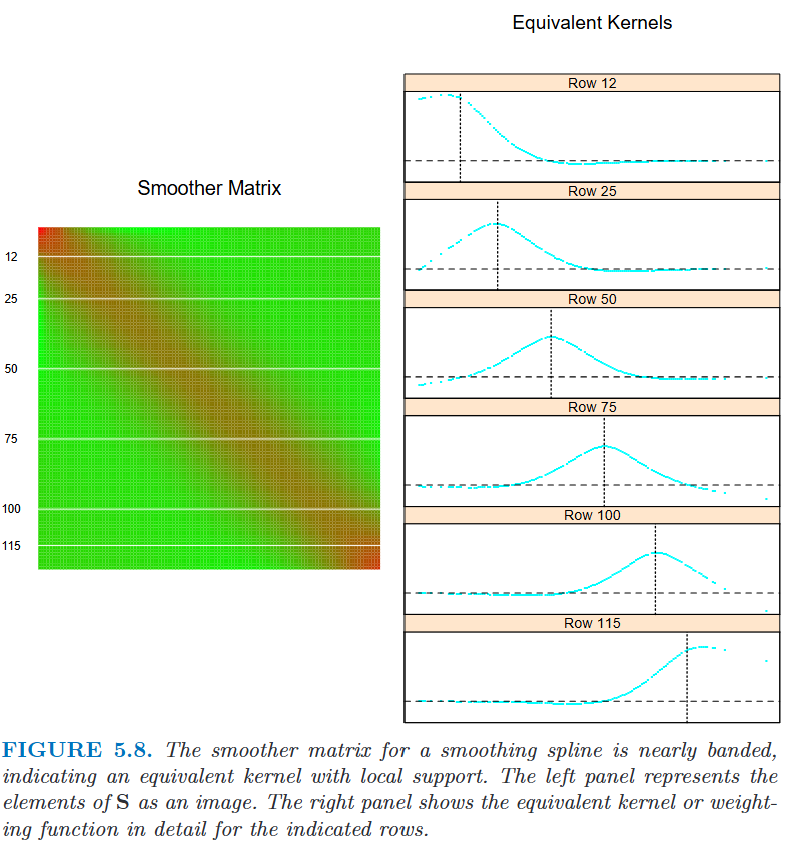
\includegraphics[width=0.85\textwidth]{Chapters/pic/ch_基展开和正则化/figure_5_8.png}
\caption{光滑样条的光滑矩阵 $\mathbf{S}_\lambda$。左：矩阵元素图（行按 $x$ 排序），带状结构表明局部支撑。右：选定行的等价核（加权函数），每行在对应 $x_i$ 处取峰值并向两侧衰减。来源：ESL Figure 5.8。}
\label{fig:smoother_matrix}
\end{figure}

图 5.8 展示了光滑矩阵 $\mathbf{S}_\lambda$ 的带状结构（行按 $x$ 排序）——表明光滑样条本质上是一个\textbf{局部拟合方法}，类似于第 6 章的局部加权回归。$\mathbf{S}_\lambda$ 的每一行即为\textbf{等价核}——$\hat{f}(x_i)$ 实质上是 $y_i$ 附近点的加权平均，权重在 $x_i$ 处最大并向两侧衰减。

\[
\lambda \to 0 \Longrightarrow \mathrm{df} \to N,\; \mathbf{S}_\lambda \to \mathbf{I}, \qquad
\lambda \to \infty \Longrightarrow \mathrm{df} \to 2,\; \mathbf{S}_\lambda \to \mathbf{H}_{\text{线性}}.
\]


% ============ §5.5 光滑参数的自动选择 ============
\section{光滑参数的自动选择}

\subsection{用有效自由度参数化}

光滑样条的 $\mathrm{df}_\lambda = \operatorname{trace}(\mathbf{S}_\lambda)$ 关于 $\lambda$ 单调递减（$\lambda$ 越大 $\to$ df 越小 $\to$ 越光滑），可以反解——\textbf{固定 df 来确定 $\lambda$}。实践中通过简单数值方法实现（如 R 的 \texttt{smooth.spline(x, y, df=6)}）。

这种方法鼓励更传统的模型选择模式：尝试几个不同的 df 值，基于近似 $F$ 检验、残差图等主观准则选择。\textbf{df 的统一度量使不同的光滑方法可以公平比较}——在广义加性模型（第 9 章）中尤其有用，多个光滑方法可同时用于一个模型。

\subsection{偏差-方差权衡}

\begin{figure}[htbp]
\centering
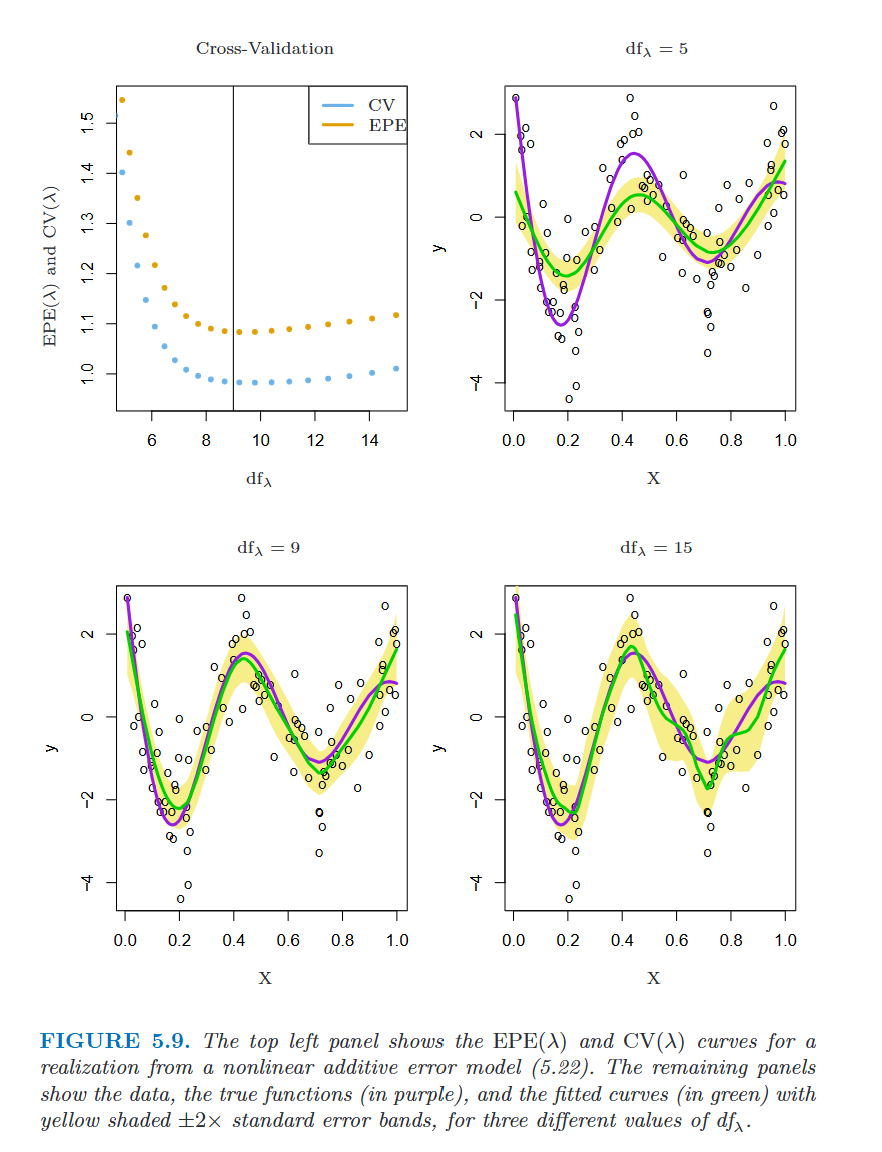
\includegraphics[width=0.95\textwidth]{Chapters/pic/ch_基展开和正则化/figure_5_9.png}
\caption{左上：EPE($\lambda$) 和 CV($\lambda$) 曲线。其余三面板：真实函数（紫色）、拟合曲线（绿色）及 $\pm 2$ 标准误带（黄色），分别对应 $\mathrm{df}=5,9,15$。$\mathrm{df}=5$ 欠拟合，$\mathrm{df}=15$ 略显过拟合，$\mathrm{df}=9$ 接近最优。来源：ESL Figure 5.9。}
\label{fig:bias_variance}
\end{figure}

图 5.9 用模拟数据 $Y = \frac{\sin(12(X+0.2))}{X+0.2} + \varepsilon$（$X \sim U[0,1], \varepsilon \sim N(0,1), N=100$）展示了 df 的三个取值：

\begin{center}
\small
\begin{tabular}{c|p{5.5cm}|p{4.5cm}}
\toprule
$\mathrm{df}_\lambda$ & 表现 & 诊断 \\
\midrule
5 & 欠拟合：削峰填谷，高曲率区偏差大 & 标准误带极窄——有偏但确信 \\
9 & 接近最优，轻微偏差 & 方差尚未明显增加 \\
15 & 略显波动，接近真实函数 & 标准误带增宽——追随个别点 \\
\bottomrule
\end{tabular}
\end{center}

\textbf{定量表达}：$\hat{\mathbf{f}} = \mathbf{S}_\lambda\mathbf{y}$ 的方差-偏差分解为
\[
\operatorname{Cov}(\hat{\mathbf{f}}) = \mathbf{S}_\lambda\mathbf{S}_\lambda^\top, \qquad
\operatorname{Bias}(\hat{\mathbf{f}}) = \mathbf{f} - \mathbf{S}_\lambda\mathbf{f},
\]
其中 $\mathbf{f}$ 是未知真实值向量。\textbf{EPE（期望预测误差）}综合了偏差和方差：
\[
\operatorname{EPE}(\hat{f}_\lambda) = \E\big(Y - \hat{f}_\lambda(X)\big)^2
= \sigma^2 + \underbrace{\E[\operatorname{Bias}^2(\hat{f}_\lambda(X))] + \E[\operatorname{Var}(\hat{f}_\lambda(X))]}_{\operatorname{MSE}(\hat{f}_\lambda)}.
\]

\subsection{交叉验证 (CV)}

$\lambda$ 的实际选择通过最小化 CV 得分：
\[
\operatorname{CV}(\hat{f}_\lambda) = \frac{1}{N} \sum_{i=1}^{N} \big( y_i - \hat{f}_\lambda^{(-i)}(x_i) \big)^2,
\]
其中 $\hat{f}_\lambda^{(-i)}$ 是删除第 $i$ 个观测后拟合的模型。对光滑样条这一线性光滑器，有\textbf{免重拟合公式}（习题 5.13）：
\[
\boxed{\operatorname{CV}(\hat{f}_\lambda) = \frac{1}{N} \sum_{i=1}^{N}
\left( \frac{y_i - \hat{f}_\lambda(x_i)}{1 - S_\lambda(i,i)} \right)^2,}
\]
即只需完整拟合一次，使用对角线元素 $S_\lambda(i,i)$ 校正。CV 曲线是 EPE 曲线的近似无偏估计量（图 5.9 左上）。\textbf{对回归样条}还需额外选择节点位置和数量——这是个组合爆炸问题，除非使用 MARS（§9.4）等贪心策略。


% ============ §5.6 非参数 Logistic 回归 ============
\section{非参数 Logistic 回归}

将光滑样条从回归推广到分类是直接了当的。对单个连续输入 $X$ 的 Logistic 回归：
\[
\log\frac{\Pr(Y=1\mid X=x)}{\Pr(Y=0\mid X=x)} = f(x), \qquad
\Pr(Y=1\mid X=x) = \frac{e^{f(x)}}{1 + e^{f(x)}}.
\]
在光滑样条框架下拟合 $f$ 得到条件概率 $\Pr(Y=1\mid x)$ 的光滑估计。

\textbf{惩罚对数似然准则}：
\begin{equation}\label{eq:penalized_loglik}
    \ell(f; \lambda) = \sum_{i=1}^{N} \big[ y_i f(x_i) - \log(1 + e^{f(x_i)}) \big]
    - \frac{\lambda}{2} \int \big\{ f''(t) \big\}^2 dt,
\end{equation}
第一项是二项分布的对数似然（第 4 章），第二项是曲率惩罚。与回归情况一样，最优 $f$ 是节点在唯一 $x_i$ 处的有限维自然样条：$f(x) = \sum_{j=1}^{N} N_j(x)\,\theta_j$。

\textbf{Newton-Raphson 迭代}：梯度和 Hessian 为
\[
\frac{\partial\ell}{\partial\boldsymbol{\theta}} = \mathbf{N}^\top(\mathbf{y} - \mathbf{p}) - \lambda\boldsymbol{\Omega}\boldsymbol{\theta}, \qquad
\frac{\partial^2\ell}{\partial\boldsymbol{\theta}\partial\boldsymbol{\theta}^\top} = -\mathbf{N}^\top\mathbf{W}\mathbf{N} - \lambda\boldsymbol{\Omega},
\]
其中 $\mathbf{W} = \operatorname{diag}(p_i(1-p_i))$。Newton 更新为：
\begin{equation}\label{eq:nplr_update_theta}
    \boldsymbol{\theta}^{\mathrm{new}} = (\mathbf{N}^\top\mathbf{W}\mathbf{N} + \lambda\boldsymbol{\Omega})^{-1}
    \mathbf{N}^\top\mathbf{W}\,\mathbf{z},
\end{equation}
或以拟合值表示：
\[
\mathbf{f}^{\mathrm{new}} = \underbrace{\mathbf{N}(\mathbf{N}^\top\mathbf{W}\mathbf{N} + \lambda\boldsymbol{\Omega})^{-1}\mathbf{N}^\top\mathbf{W}}_{\mathbf{S}_{\lambda,w}} \mathbf{z}
    = \mathbf{S}_{\lambda,w}\,\mathbf{z}.
\]
这恰好是\textbf{加权光滑样条}对工作响应 $\mathbf{z}$ 的拟合——与 §4.4.1 的 IRLS 完全一致，只是将线性回归换成了光滑样条。

\textbf{推广}：$\mathbf{S}_{\lambda,w}$ 可替换为任何非参数（加权）回归算子，得到一般的非参数 Logistic 回归族。该思想自然推广到高维——这正是\textbf{广义加性模型（GAM，第 9 章）}的基石。


% ============ §5.7 多维样条 ============
\section{多维样条}

至此所有样条均为一维。本节讨论多维推广。

\subsection{张量积基}

设有一维基函数族 $\{h_{1j}(X_1)\}_{j=1}^{M_1}$ 和 $\{h_{2k}(X_2)\}_{k=1}^{M_2}$，则 $M_1 \times M_2$ 维\textbf{张量积基}定义为：
\begin{equation}\label{eq:tensor_product}
    g_{jk}(X) = h_{1j}(X_1)\,h_{2k}(X_2), \quad j=1,\ldots,M_1,\; k=1,\ldots,M_2,
\end{equation}
二维函数表示为：
\[
g(X) = \sum_{j=1}^{M_1}\sum_{k=1}^{M_2} \theta_{jk}\,g_{jk}(X).
\]
图 5.10 展示了使用 B-样条的张量积基。系数由最小二乘拟合。

\textbf{可推广到 $d$ 维}，但基的维度指数增长——\textbf{维数灾难的又一个表现}。MARS（§9.4）使用贪心前向算法仅包含最小二乘认为必要的张量积项。

\textbf{加性 vs 张量积}：图 5.11 比较了二维分类问题上两者的决策边界。加性模型（各自样条相加）捕捉主效应，张量积可拟合更灵活的交互，但可能引入虚假结构。

\subsection{薄板样条 (Thin-Plate Splines)}

一维光滑样条的正则化思想可推广到 $\R^d$：
\begin{equation}\label{eq:thin_plate}
    \min_{f} \sum_{i=1}^{N} \big\{ y_i - f(x_i) \big\}^2 + \lambda J[f],
\end{equation}
其中 $J[f]$ 是 $d$ 维粗糙度惩罚。对 $d=2$：
\[
J[f] = \iint_{\R^2} \left[ \left(\frac{\partial^2 f}{\partial x_1^2}\right)^2
    + 2\left(\frac{\partial^2 f}{\partial x_1\partial x_2}\right)^2
    + \left(\frac{\partial^2 f}{\partial x_2^2}\right)^2 \right] dx_1 dx_2.
\]

\textbf{解的形式}（与一维自然三次样条共享性质）：
\[
f(x) = \beta_0 + \boldsymbol{\beta}^\top x + \sum_{j=1}^{N} \alpha_j\,h_j(x),
\quad h_j(x) = \|x - x_j\|^2 \log\|x - x_j\|,
\]
其中 $h_j$ 为\textbf{径向基函数}（§5.9 详述）。系数由带线性约束的惩罚最小二乘确定（习题 5.14）。
\[
\lambda \to 0 \Rightarrow \text{插值表面}, \qquad
\lambda \to \infty \Rightarrow \text{最小二乘平面}.
\]

\textbf{计算复杂度}：薄板样条为 $O(N^3)$（一般无稀疏结构可资利用），实践中用放置在一组格点上的\textbf{节点约简}：用 $K$ 个节点将计算量降至 $O(NK^2 + K^3)$。图 5.12 展示了心脏病数据上年龄 × 肥胖的薄板样条拟合（$\mathrm{df}=15$）。

\subsection{加性样条与 ANOVA 分解}

多维样条的一类重要限制是\textbf{加性模型}：
\[
f(X) = \alpha + f_1(X_1) + f_2(X_2) + \cdots + f_d(X_d),
\]
每 $f_j$ 是一维样条。惩罚自然施加于各分量：
\[
J[f] = \sum_{j=1}^{d} \int f_j''(t_j)^2\,dt_j.
\]
这自然推广到 ANOVA 分解：
\[
f(X) = \alpha + \sum_j f_j(X_j) + \sum_{j<k} f_{jk}(X_j, X_k) + \cdots,
\]
每项为相应维数的样条。需做的选择包括：最大交互阶数、包含哪些项、每项使用回归样条还是光滑样条。MARS（§9.4）和 MART（第 10 章）提供了自动化方案。


% ============ §5.8 正则化与再生核 Hilbert 空间 ============
\section{正则化与再生核 Hilbert 空间 (RKHS)}

本节将样条纳入正则化方法的更广阔框架。

\subsection{一般形式}

一类正则化问题可统一写为：
\begin{equation}\label{eq:general_regularization}
    \min_{f \in \mathcal{H}} \left[ \sum_{i=1}^{N} L(y_i, f(x_i)) + \lambda J(f) \right],
\end{equation}
其中 $L$ 为损失函数，$J(f)$ 为惩罚泛函，$\mathcal{H}$ 为 $J(f)$ 有定义的函数空间。

若惩罚在 Fourier 域中取形式 $J(f) = \int |\tilde{f}(s)|^2 / \tilde{G}(s)\,ds$（$\tilde{G}$ 在高频处衰减），则解具有有限维表示：
\[
f(X) = \sum_{k=1}^{K} \alpha_k \phi_k(X) + \sum_{i=1}^{N} \theta_i G(X - x_i),
\]
其中 $\phi_k$ 张成惩罚的零空间（不惩罚的方向），$G$ 是 $\tilde{G}$ 的 Fourier 逆变换。光滑样条和薄板样条均属此框架。

\subsection{RKHS 与核方法}

一个重要子类由\textbf{正定核} $K(x, y)$ 生成。相应函数空间 $\mathcal{H}_K$ 称为\textbf{再生核 Hilbert 空间}。设核的特征展开为 $K(x,y) = \sum \gamma_i \phi_i(x)\phi_i(y)$，则范数定义为 $\|f\|_{\mathcal{H}_K}^2 = \sum c_i^2/\gamma_i$，其中 $f = \sum c_i\phi_i$。惩罚取 $J(f) = \|f\|_{\mathcal{H}_K}^2$。

\textbf{表示定理 (Representer Theorem)}：问题
\[
\min_{f \in \mathcal{H}_K} \sum_{i=1}^{N} L(y_i, f(x_i)) + \lambda \|f\|_{\mathcal{H}_K}^2
\]
的有限维解为：
\[
\boxed{f(x) = \sum_{i=1}^{N} \alpha_i K(x, x_i)}.
\]
且 $J(f) = \boldsymbol{\alpha}^\top \mathbf{K} \boldsymbol{\alpha}$（$\mathbf{K}_{ij} = K(x_i, x_j)$）。无穷维优化 $\Rightarrow$ $N$ 维问题 $\min_{\boldsymbol{\alpha}} L(\mathbf{y}, \mathbf{K}\boldsymbol{\alpha}) + \lambda \boldsymbol{\alpha}^\top\mathbf{K}\boldsymbol{\alpha}$。

\textbf{更一般的分解} $\mathcal{H} = \mathcal{H}_0 \oplus \mathcal{H}_1$：$\mathcal{H}_0$（多项式零空间，不惩罚）$+$ $\mathcal{H}_1$（惩罚空间）。解为 $f(x) = \sum_{j} \beta_j h_j(x) + \sum_{i} \alpha_i K(x, x_i)$。

\subsection{实例}

\textbf{平方误差损失}：$\hat{\boldsymbol{\alpha}} = (\mathbf{K} + \lambda\mathbf{I})^{-1}\mathbf{y}$，$\hat{\mathbf{f}} = \mathbf{K}(\mathbf{K} + \lambda\mathbf{I})^{-1}\mathbf{y} = (\mathbf{I} + \lambda\mathbf{K}^{-1})^{-1}\mathbf{y}$（对比光滑样条的 $(\mathbf{I}+\lambda\mathbf{K})^{-1}\mathbf{y}$）。在空间统计中称为 Kriging 估计。

\textbf{多项式核}：$K(x,y) = (\langle x,y\rangle + 1)^d$。$M = \binom{p+d}{d}$ 个基函数（可能 $\gg N$），但核表示只需 $O(N^3)$——这是\textbf{核技巧}的本质：隐式使用高维特征空间而不显式构造它。

\textbf{高斯径向基核}：$K(x,y) = e^{-\nu\|x-y\|^2}$。每个基函数 $k_m(x) = K(x, x_m)$ 是以训练点 $x_m$ 为中心的 Gaussian。核尺度 $\nu$ 控制局部性：$\nu$ 越大 $\to$ 越局部 $\to$ 有效维数越高（图 5.14--5.15）。

\textbf{薄板样条核}：$K(x,y) = \|x-y\|^2\log(\|x-y\|)$（径向基函数形式的薄板样条）。

\textbf{支持向量机}（第 12 章）：二分类下使用 hinge loss：
\[
\min_{\alpha_0, \boldsymbol{\alpha}} \sum_{i=1}^{N} [1 - y_i f(x_i)]_+ + \frac{\lambda}{2}\boldsymbol{\alpha}^\top\mathbf{K}\boldsymbol{\alpha},
\]
非零 $\hat{\alpha}_i$ 对应的 $x_i$ 即为\textbf{支持向量}。


% ============ §5.9 小波光滑 ============
\section{小波光滑}

小波提供了一种与样条互补的基函数字典：样条通过\textbf{光滑性}实现压缩，小波通过\textbf{稀疏性}实现压缩。

\subsection{核心思想：时间-频率定位}

样条擅长表示光滑函数（用少量基函数）；小波擅长表示「大部分平坦 + 少数突起」的信号（用少量 bumpy 基函数）。小波基能同时定位\textbf{时间}（突起在哪里）和\textbf{频率}（突起有多尖锐）——传统 Fourier 基只能定位频率。

\subsection{多分辨率分析}

小波基通过单个\textbf{尺度函数} $\phi(x)$（父小波）和\textbf{母小波} $\psi(x)$ 的平移和缩放生成。以 Haar 小波为例：
\[
\phi(x) = I(0 \le x < 1), \qquad
\psi(x) = \phi(2x) - \phi(2x-1) \;\;(\text{在}[0,\tfrac12)\text{为}+1,\;[\tfrac12,1)\text{为}-1).
\]

空间分解：$V_{j+1} = V_j \oplus W_j$（$V_j$ = 分辨率 $2^{-j}$ 的逼近空间，$W_j$ = 细节空间）。迭代得\textbf{多分辨率分解}：
\[
V_J = V_0 \oplus W_0 \oplus W_1 \oplus \cdots \oplus W_{J-1}.
\]
$V_0$ 是最粗逼近（Haar 下为常数），$W_0, W_1, \ldots$ 是递增分辨率的细节层。

Haar 基简单但不光滑，实践中更常用\textbf{symmlet-p} 族：
\begin{itemize}
    \item 支撑：$2p-1$ 个连续区间（Haar 为 1）；
    \item 消失矩：$p$ 个（$\int \psi(x)x^j dx = 0,\; j=0,\ldots,p-1$），使 $V_0$ 可精确复现 $p$ 阶多项式——类比光滑样条惩罚的零空间。
\end{itemize}

\subsection{自适应小波阈值 (Wavelet Shrinkage)}

对一维离散信号 $\mathbf{y}$（$N=2^J$ 均匀样本），设 $\mathbf{W}$ 为 $N \times N$ 正交小波基矩阵，\textbf{小波变换} $\mathbf{y}^* = \mathbf{W}^\top \mathbf{y}$ 给出每个基上的系数。

SURE 收缩（Donoho \& Johnstone, 1994）求解 Lasso 型问题：
\[
\min_{\boldsymbol{\theta}} \|\mathbf{y} - \mathbf{W}\boldsymbol{\theta}\|^2 + 2\lambda \|\boldsymbol{\theta}\|_1.
\]
由于 $\mathbf{W}$ 正交，解有显式\textbf{软阈值}规则：
\begin{equation}\label{eq:soft_threshold}
    \hat{\theta}_j = \operatorname{sign}(y_j^*)\,(|y_j^*| - \lambda)_+.
\end{equation}
即将系数向零平移 $\lambda$，不足 $\lambda$ 的置为零。常用阈值 $\lambda = \hat{\sigma}\sqrt{2\log N}$——理由：$N$ 个白噪声变量的最大绝对值约为 $\sigma\sqrt{2\log N}$，低于此的系数大概率是噪声。

逆小波变换 $\hat{\mathbf{f}} = \mathbf{W}\hat{\boldsymbol{\theta}}$ 得光滑后信号。

\subsection{小波 vs 光滑样条（图 5.17, 5.19）}

\begin{center}
\begin{tabular}{lll}
\toprule
& 光滑样条 & 小波收缩 \\
\midrule
适应对象 & 整体光滑的信号 & 平坦+局部尖峰的信号 \\
压缩方式 & 曲率惩罚→光滑 & $\ell_1$ 阈值→稀疏 \\
计算 & $O(N)$ & $O(N)$（金字塔算法，比 FFT 更快） \\
\bottomrule
\end{tabular}
\end{center}

图 5.17 的 NMR 信号演示了完整流程：原始信号 → 小波变换（系数按尺度排列）→ 软阈值去噪 → 逆变换重建。

图 5.19 对比了两类信号的拟合：NMR 尖峰信号中小波优于样条（精确定位尖峰，样条为迁就尖峰在整个域引入多余波动）；光滑信号中样条优于小波（小波为获得自适应性付出了额外方差的代价）。\textbf{两者的选择取决于信号的光滑 vs 稀疏性质。}

\begin{remark}
二维小波是现代图像压缩（如 JPEG2000）的核心技术。本章参考文献见 de Boor (1978)、Wahba (1990)、Daubechies (1992)、Donoho \& Johnstone (1994) 等。
\end{remark}
